\documentclass[a4paper,12pt]{article}
\usepackage[utf8]{inputenc}
\usepackage{amsmath}
\usepackage{amsfonts}
\usepackage{amssymb}
\usepackage{graphicx}
\usepackage{listings}
\usepackage{color}
\usepackage{hyperref}
\usepackage[romanian]{babel}

\title{Stomadmin - Managementul unui cabinet stomatologic}
\author{Alexandru Munteanu\\
Darius Petrov\\
Ioan Samuilă\\
Departamentul de Informatică\\
Facultatea de Matematică și Informatică\\
Universitatea de Vest din Timișoara}
\date{}

\begin{document}

\maketitle
\begin{abstract}
Stomadmin este o aplicație de managemet a fluxurilor de activități dintr-un cabinet stomatologic.

 În principal, gestionează evidența pacienților și a consultațiilor acordate acestora din punct de vedere al diagnosticării și medicației prescrise. 

Păstrează o evidența a consultațiilor, trimiterilor și a altor documente medicale cum ar fi de exemplu, scrisorile medicale.  
\end{abstract}

\pagebreak

\tableofcontents

\pagebreak

\section{Introducere}

Stomadmin este o aplicație dezvoltată cu ajutorul tehnologiilor web și utilizează pentru rulare sistemul client - server.

Într-o bază de date sunt păstrate înregistrările ce privesc activitățile medicale specifice unui cabinet stomatologic, iar această bază de date este găzduită de un server care se poate afla în locația clientului sau într-o alta locație.

Principalele tehnologiile folosite în procesul de dezvoltare sunt:

\begin{itemize}
\item PHP 7
\item Bootstrap 4
\item Laravel 5.x
\item MySQL
\item Git (github.com)
\end{itemize}

Accesarea datelor se face cu ajutorul unui browser web și permite diferite niveluri de acces. În principal vorbim de următoarele tipuri de conturi:

\begin{itemize}
\item Administrator
\item Medic Specialist
\item Secretară
\item Pacient
\end{itemize} 

Funcționalitățile aplicației pot fi testate la adresa: \url{https://erdt.ddns.net} , unde se află o varianta demo a proiectului ce conține un set de utilizatori și inregistrări fictive.

În capitolele ce urmează va fi prezentat mai pe larg felul în care utilizatorii menționați mai sus interacționează cu sistemul.

\section{Funcționalități}

Pentru accesarea panoului prorpriu de control utilizatorul trebuie să introduca un nume de utilizator și o parolă. În funcție de credențialele introduse, sistemul recunoaște tipul de utilizator care a accesat sistemul și îi oferă acces către funcțiile predefinite specifice ale acestuia.

Pentru o imagine cât mai completa asupra sistemului, în figura~\ref{fig:home} este prezentată interfața ce se afieșază in cazul conectării cu un cont de administrator.  

\begin{figure}[h]
\centering
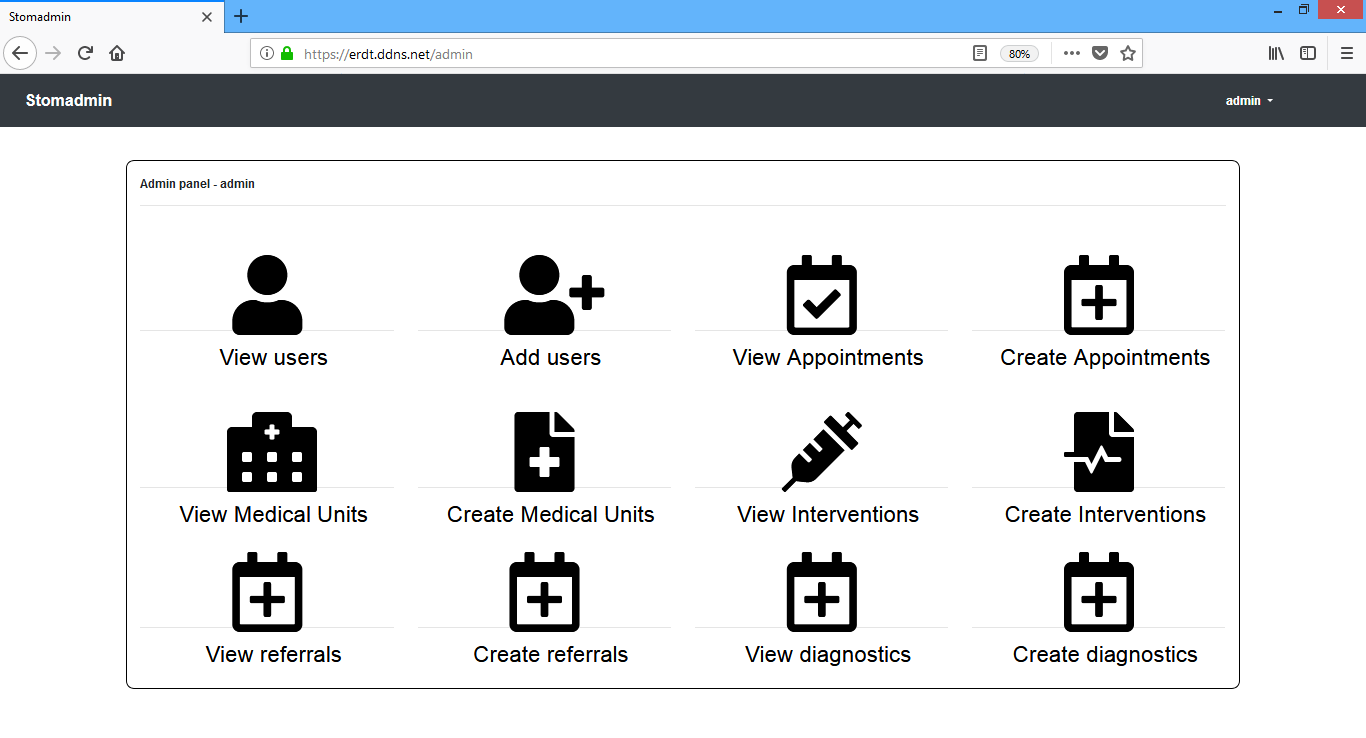
\includegraphics[width=5in]{home}
\caption{Interfața utilizatorului}
\label{fig:home}
\end{figure}

\section{Tipuri de utilizatori}

Așa cum am menționat și anterior grupurile de utilizatori care sunt predefiniți în aplicație sunt împărțiți în următoarele categorii:
\begin{itemize}
\item Administrator
\item Medic Specialist
\item Secretară
\item Pacient
\end{itemize}

\subsection{Administrator}

Administratorul are control deplin asupra sistemului. Aadar adminstratorul(sau administratorii,  în funcție de solicitare) sitemului are(au) următoarele drepturi:

\begin{itemize}
\item  poate să creeze conturi de doctor, secretară și pacient;
\item poate modifica tarifele consultațiilor și intervențiilor pentru pacienți;
\item poate să vadă bilanțul încasăriilor pe cabinet cât și pe doctor și să genereze diferite statistici.
\item poate adăuga, șterge sau bloca utilizatori.
\end{itemize}

\subsection{Medic Specialist}

Medicul specialist are drepturi de editare și vizualizare a datelor, astfel el poate opera următoarele modificări:

\begin{itemize}
\item vede ce pacient are programat în ziua respectiva și completează foaia de consult;
\item poate sa facă trimitere către spital, laborator și radiologie;
\item poate sa elibereze o scrisoare medicala către medicul de familie în care sa precizeze diagnosticul și investgiația despre pacient cât și medicamentele prescrise;
\item la finalul consultului bifează tipurile de intervenții făcute;
\end{itemize}

\subsection{Secretara}

Secretara de asemena este un utilizator cu drepturi atât de scriere căt și de citire. Prin urmare acest tip de utilizator poate manipula următoarele date:

\begin{itemize}
\item programează pacientul la un doctor și îl înregistrează la cabinet;
\item poate sa anuleze programarea unui pacient sau sa o modifice pe alta data;
\item poate să vadă consultul pacientului și trimiterile către laborator, spital și radiologie, cât și biletul de plata;
\item  si poate să imprime toata fisa pacientului sau o parte cat si biletul de plata.
\item poate sa faca contabilitatea pe doctor/ doctori atat pe zi cat si pe luna si an.
\end{itemize}

\subsection{Pacient}

Acest tip de cont este un tip de cont simplu care nu are drepturi de modificare asupra sistemului ci doar de vizualizare. Accesul în sistem se face pe baza unui nume de utilizator și a unei parole.

Pacientul are acces la rezultate, la interpretarea lor şi la recomandările medicului.

\section{Concluzii}

Aplicația Stomadmin se adresează în principal cabinetelor de dimensiune mică însă este dezvoltată modular astfel încât permite modificarea ulterioară prin adăugarea de noi module în funcție de necesitățile utilizatorului.

În cazul unei solicitări se pot modifica drepturile de acces, se pot adăuga tipuri de utilizatori noi cu drepturi de acces noi. Acest lucru însă se poate realiza doar la nivel de modificare al codului, nu din interfață utilizator.

\end{document}